In this section, we cover the main design issues for the \muemat\ \operator class.
An \operator is simply a matrix whose data is either owned by an application or by \muemat.
The data may be stored in \point or block form, but this is secondary to how the \operator will be accessed.
Accessibility is arguably the more important consideration because all phases of setup and solve require
\operator operations. Access requirements may change from one phase to the next, due to algorithmic
reasons.  However, using a view different than the native storage format  may incur a significant performance penalty.

\subsubsection{When One View Just Isn't Enough}
The most common format for an \operator will almost certainly be the \point compressed row storage format, also known as
CRS.
Some matrices may be stored in a block format, but this will probably be much rarer.

Once an \operator is constructed, however, we want the ability to access it as if it were stored in some format other
than its native storage format.
There appear to be two main use cases:
\be
  \item The matrix is stored natively as a \point CRS matrix.  Point and block \getrow access are required.
  \item The matrix is stored natively as a block matrix.  Either \point access\footnote{This is an expensive operation.  Blocks
  are likely stored as small dense matrices or as the fundamental scalar type.  In either case, this involves lots of
  indirect lookups and copies.} or block access with a different size block is required
  \footnote{This could be expensive if the requested block size is larger 
  than but not evenly divisible by the smaller native size, or if the requested block size is smaller than the native
  size.}.
\ee
These could occur, for example, in smoothers like Gauss-Seidel that need \getrow access,
in aggregation during the setup of the prolongator, or in a matrix-matrix multiply.
Figure \ref{operator feature matrix} summarizes the combination of native format and view possibilities.
%
\begin{figure}[tbhp]
  \centering
  % format | NativeView PointView DifferentlyBlockedView InsertDifferentFromNative
  \begin{tabular}{|c|cc|cc|}
    \hline
    &  \multicolumn{2}{c|}{View} & \multicolumn{2}{c|}{Insert}\\\cline{2-5}
    \raisebox{1.5ex}[0cm][0cm]{Native format} 
      %    |       View         |      Insert     |
           &  \block  & \point &  \block  & \point\\ \hline
    \block &    Y$^\dagger$ &   Y   &     Y$^\dagger$    &    ?  \\ \hline
    \point &    Y     &   Y   &     N    &    Y  \\ \hline
  \end{tabular}\\
  $^\dagger${\small Includes different blocking than native format}
\caption{\label{operator feature matrix}Operator row access feature matrix.}
\end{figure}\\

\noindent
Here are a couple comments on matrix views.\\

\noindent
{\bf Point Views}:  This is the easier case, albeit more expensive.  For a matrix stored in a block format, we wish to
extract a \point row.  This requires determining the block row that contains the \point row.  Then it is just a matter of
extracting the correct point row.

\noindent
{\bf Block Views}:  First suppose the matrix is natively in \point format.  If the matrix is thought instead to be of
constant block size, then this is a simple lookup of the correct point rows and translation into dense block entries.

%There is at least one map initially associated with an \operator, namely, the row map provided when it is constructed.
%There are also other maps that are constructed internally when the matrix is transformed from global to local numbering
%and data transfer patterns are created -- the column, domain, and range maps.  For purposes of this discussion, however,
%the row map is the most important of the maps. \JJH{I think....}

%Once the \operator is constructed, however, it should be possible to access it with a different yet compatible map.
%Once the \operator is constructed, however, we may want to have different views of the matrix:
%
%\be
%    \item Native point matrix
%    \be
%      \item point getrow
%      \item block getrow
%    \ee
%    \item Native block matrix
%    \be
%      \item point getrow -- This is an expensive operation.  Blocks are likely stored as small dense matrices or
%      as the fundamental scalar type.  In either case, this involves lots of indirect lookups and copies.
%      \item different block getrow -- This could be expensive if the smaller block size does not evenly divide the larger.
%    \ee
%\ee
%
%\JJH{Define ``compatible" map.}
%For example, suppose we have a \point\ \operator $A$ with 5 rows, numbered 0 to 4.  $A$ should be compatible with a block
%map that contains 2 elements, the first with 3 point entries and the second with 2 point entries, as long as the global
%numbering is the same.
%In general, one can imagine accessing an \operator with many different compatible maps.  

\subsubsection{Multiple Diagonals}

For both relaxation and prolongator smoothing, we may want to experiment with different types of diagonals.
An operator could have associated with it more than one \point diagonal (e.g., the true \point diagonal and a lumped
version) and more than one block diagonal (differently sized blocks, same sized blocks but different values).
Furthermore, the blocks in the diagonal might be distributed, e.g., if we are solving a blocked system
$$ \left[ \begin{array}{cc} A & B \\ C & D \end{array} \right], $$
a block diagonal entry $d_{ii}$ might consist of \point entries from all four blocks:
$$d_{ii} = \left[ \begin{array}{cc} a_{ii} & b_{ii} \\ c_{ii} & d_{ii} \end{array} \right].$$
%
We may also want to play with overlapped block diagonals, such as for Arnold-Falk-Winther smoothing.

\noindent
{\bf Questions}
\be
\item The most reasonable place for the diagonals to be stored is with the operator.  How do we indicate
that we want to use a particular one?  How do we check to see whether a particular diagonal is present?
%
\item Should we be able to register a new diagonal at anytime?  If so, how do we go about this? Or, should we only
be able to construct the diagonals when the operator is built?
%
\item When we define a diagonal, this fixes the row map.  Does there have to be a \getrow that corresponds to this map?
\ee

\subsubsection{Other Considerations}

We may also want to be able to do a deep copy of a matrix from one storage type to another.
This means that we'll need converters from \point to block and vice-versa.\\

\subsubsection{An \operator strawman}

\be
\item The \operator must have pairs of \getrow{s} and diagonals.  It is not possible to have a \getrow without a
corresponding diagonal, or vice-versa.

\item The \operator has a ``state" manager that remembers the current view of the matrix and is the only way
to change the view.

\ee

\noindent
{\bf Comment}:  One design possibility is to {\em always} store the matrix as a CSR matrix, and only use views to access
it as a block matrix.  This means giving up performance, but simplifies our interactions with 3rd party linear algebra
packages.


\subsection{Current design of \Operator related classes}
Figure \ref{fig:current:OperatorClassDiagram} presents the current design of the \Operator class. Note that only the classes \Operator and \Diagonal are directely used on the other parts of \muemat.
SetXXX() methods are not represented on this diagram. The \Map class is also missing.

\begin{figure}
\centering  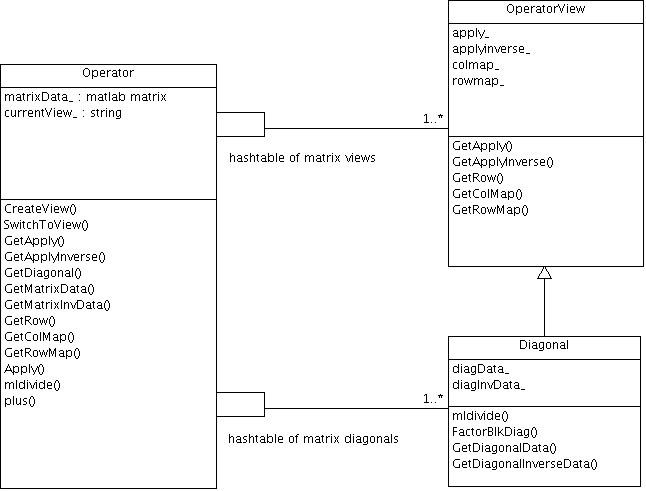
\includegraphics[angle=90,width=0.8\textwidth]{figs/MueMatOperatorClassDiagram.png}
  \caption{Class diagram of \Operator classes.}
  \label{fig:current:OperatorClassDiagram}
\end{figure}

\subsubsection{The \Operator class}
An \Operator is simply a matrix. In \muemat, the matrix data are natively stored as a MATLAB matrix (encapsulated in the \Operator object) and you can access directly to internal data storage by using the method GetMatrixData().
This accessor is used in \muemat for convenience and efficiency reasons.\\

Some \muemat algorithms mimic the fact that we only have such row accessors: These algorithms loops over the rows and blocks and extract blocks from the MATLAB matrix:

\subsubsection{The view mecanism}

One goal of the \Operator class is to be a thin interface layer between Epetra/Tpetra and \mloo (to allow us to be compatible with both libraries).
An other important goal is the ability to access matrix as if it were stored in some format other than its native storage format.
For example, we would like to be able to access block matrices as if they were stored in a point entry storage formats or with another block size. 
Each matrix format is called a \View and the defaut view of an \Operator is the native data format of the matrix. Additional ``virtual'' views can be defined to
describe the way we want to access the data of an operator.
The views of an \Operator are stored in a \ViewTable which is just a list of \View. Each view is fully described by two Map objects (for row and columns).

\begin{remark}
At the moment, if we want to do an operation between two Operator (let's say OpA+OpB) with different internal data storage, we cannot. There is no mecanism to do that.
The easiest way to perform such operation is to use the point format as the common language between operator (slow). A better way is to find the ``greatest common block format''.
Maybe we can use a method to compare Maps:
\begin{verbatim}
function Operator::Add(OperatorA,OperatorB)

  CommonView = View.GetCommonView(OperatorA.DefaultView(), 
                                  OperatorB.DefaultView());
  OperatorA.AddView('tmpView',CommonView);
  OperatorB.AddView('tmpView',CommonView);
  
  oldAview = OperatorA.SwitchToView('tmpView');
  oldBview = OperatorB.SwitchToView('tmpView');
  
  \% loop to perform A+B
  for() 

  end

  OperatorA.DeleteView('tmpView'); 
  OperatorB.DeleteView('tmpView'); 

  OperatorA.SwitchToView(oldAview);
  OperatorB.SwitchToView(oldBview);
end
\end{verbatim}
% note: view should not be own by an Operator,use instead handle...
\end{remark}

For \ViewTable, what we need is \textbf{just} an hash table to get and set \View of an \Operator.
  
\subsubsection{The \Diagonal class}

In \mloo, we would like to be able to use several format of diagonal (block diagonal, point diagonal \dots). So, the View mecanism is also implemented for \Diagonal.

\begin{remark}
\ViewTable is currently a list of struct with three fields:
\begin{itemize}
\item viewLabel\_
\item matrixView\_
\item diagonalView\_
\end{itemize}
So, there is a direct relation between the view of a Diagonal and the view of the Matrix.
I think that it is better if we manage two separate list: one for diagonal view and one for matrice view.
Very specific diagonal can be created for the smoothing process. In Smoother.m, a 'Collection' can be use to define how to group blocks together for the smoothing process.
\end{remark}

%TODO: describe Operator attributes rowmapPtr_ applyFctHandle_ (avoid indirection)
% Is it interesting to have this capability in MATLAB ?

\MeetingSummary
\subsection{Summary from the March 23rd, 2010 meeting}

Key operations that could impacted by the \operator format are
\be
    \item relaxation
    \item matrix/matrix multiplication
    \item matrix/matrix addition.
    \item constraint manager
\ee
%
An \operator in \mloo should satisfy the following:
%
\be
  \item It will have a \point\ \getrow, \point diagonal, and associated data (e.g., eigenvalue estimate for $D^{-1}A$).

  \item By default, it will be stored natively as a \point matrix.  If for some reason, we want block storage, it must
  be explicitly converted.  Here is an example:

  \be
    \item User supplies $Ax=b$, all stored in constant block form.
    \item \mloo amalgamates $A$ and aggregates on the point matrix (graph, really), yielding a tall skinny point matrix
    $B$.
    \item $B$ is factored via $QR$ into two matrices, $P^{tent}$ and $N_H$, both in point format.
    \item If we want $P^{tent}$ to be in block form, we must do an explicit conversion.
    \item \JJH{An $RAP$ involves two \point matrices and one \block matrix.  I guess the result should be a \point
    matrix?}
  \ee

  One exception to this is that the result of multiplying or adding two block matrices should be a block matrix.  This
  makes sense, as both operations occur in a linear algebra library outside of \mloo.

  \item It may or may not have a block \getrow, \block diagonal, and associated data.

  \item Determining whether an \operator is compatible with another \operator reduces to determining whether the row maps
  are compatible.  Compatible means that the data distribution and ordering is the same for both maps.  Compatibility
  checks should ideally be done in the linear algebra library (or in the linear algebra interface).
  \JJH{
  I still do not think that {\em compatibility} is sufficient.  Suppose I have two serial identity matrices, one
  stored as a point matrix, $I_p$, and one as a $2\times2$ block matrix, $I_b$.  Further, suppose both have the natural
  ordering and contain the same number of point rows.
  If I want $I_p + I_b$, I must view $I_b$ as a point matrix with a point row map, even though $I_b$'s block
  row map is compatible with $I_p$'s row map.
  }

\ee
%%\end{comment} % end of \MeetingSummary

\MeetingSummary
\subsection{Summary from the August 24th, 2010 meeting, with the ZOLTAN team}

The Zoltan team is also interested to write a thin layer between Epetra/Tpetra and their future package, \zulu\footnote{Chris lobbies intensively the Zoltan team to name their next-gen package in line with \mulu. It's not clear if it worked.}.
We discussed whether it makes sense for us to collaborate on a general linear algebra interface. The needs of \zulu are focus on graph class and more limited than \mulu. 
It is not clear if writting in common the layer is of interest. So, above all, the plan is to summerize the capabilities we expect to get from such layer in writing (in this document) and pass the document to the Zoltan team.

% Zoltan also interested in being compatible with PETSc.

Mike Heroux pointed out to Jonathan that an interface package already exist in Trilinos (Thyra). It does'nt fit your needs, but we should keep that in mind (for example, if we would like to release the code of this interface separatly).
The Belos package also use a layer between the linear algebra package and itself. Needs of Belos are also very limited. It only needs a layer for vector objects and Operator object only have to provide an Apply method. The implementation of the layer uses Traits.

%%\end{comment} % end of \MeetingSummary

\MeetingSummary
\subsection{Summary from the August 24th, 2010 meeting}

During this meeting, we discuss several issues with the design of the operator class on the basis of the document known as ``10 remarks about the Operator class ...''.
Main issues concernes \mulu and how to interoperate with Epetra, Petra, IFPACK and TIFPACK. The discussion about these issues have been moved to the corresponding parts of this documents.
For the record, here are the summary of minor problems we discussed during the meeting:

\subsubsection{Old class diagram of \Operator classes}

\begin{figure}
\centering  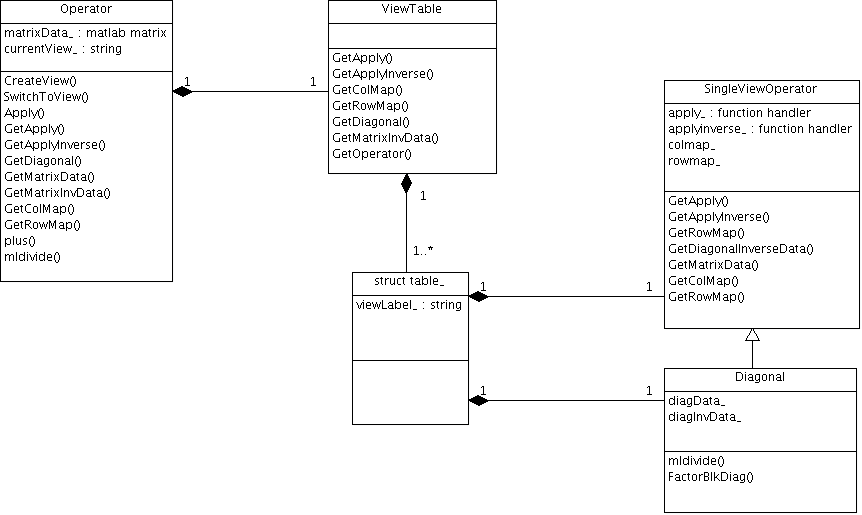
\includegraphics[angle=90,width=0.8\textwidth]{figs/bkp/MueMatOperatorClassDiagram.png}
  \caption{Class diagram of \Operator classes.}
  \label{fig:old:OperatorClassDiagram}
\end{figure}

\subsubsection{\muemat GetRow/GetBlockRow accessors}
\begin{verbatim}
nRowBlk = op.GetRowMap().NNodes();
nColBlk = op.GetRowMap().NNodes();

if op.GetRowMap().HasVariableBlkSize()

  VarRowBlkPtr = op.GetRowMap().Vptr();
  VarColBlkPtr = op.GetColMap().Vptr();
  for i=1:nRowBlk
    fRow = VarRowBlkPtr(i);
    lRow = VarRowBlkPtr(i+1)-1;
    
    for j=1:nColBlk
      fCol = VarColBlkPtr(j);
      lCol = VarColBlkPtr(j+1)-1;
      
      currentBlock = Amat(fRow:lRow, fCol:lCol);
    end % for j
  end % for i
end
\end{verbatim}
 
\begin{remark}
I think we should provide a GetRow/GetBlockRow accessors in \muemat \Operator to rewrite such algorithms more like they will be written in \mloo.
\end{remark}


\subsubsection{function handles for ApplyFunc/InvApply}

\begin{remark}
I don't understand why we use function handles for ApplyFunc/InvApply functions. In a object oriented design, we can instead implement an Operator subclass for each internal data storage.
\end{remark}

\subsubsection{Views}

\begin{remark}
I propose to rename the class \oldSingleViewOperator\blabla{ to \View because \oldSingleViewOperator is \textbf{not} an Operator. 
In fact, \oldSingleViewOperator is just an internal data structure for an operator to store the view descriptions.
\oldSingleViewOperator class was initialy design as an operator class with only one view (ie: \Operator=MultipleViewOperator),
but :
\begin{itemize}
\item A \oldSingleViewOperator is not self-sufficient (no data storage).
\item There is not inheritence relation between \oldSingleViewOperator
      and \Operator. These classes should at least implements the same
      interface.
\end{itemize}
}

\noindent \textbf{$\Rightarrow$ has been renamed \OperatorView.}
\end{remark}

\begin{remark}
\ViewTable should be only a very basic data structure. What we need is \textbf{just} an hash table to get and set \View of an \Operator.
In my opinion,the ViewTable implementation is much too heavy: Each method of \oldSingleViewOperator are
reimplemented in \ViewTable to provide a direct accessor to the \oldSingleViewOperator object properties corresponding to the requested \View.
\end{remark}

\subsubsection{Diagonal}
  
\begin{remark}
I recently added the \Diagonal class to \muemat. Initialy, we planned to use \oldSingleViewOperator class to store diagonals but 
in my opinion, there is to much diagonal specific code in MueMat (the stuff previously in src/Diag for extracting, creating, inverting diagonals) and it makes more sense to have a \Diagonal class.
\end{remark}

\begin{remark}
In Smoother.m, a 'Collection' can be use to define how to group blocks together for the smoothing process.
At the moment, this diagonal is stored as the current diagonal but a special view should be created for such specific diagonal (and there is not directely related matrix view for this diagonal).
\end{remark}

\begin{remark}
Methods GetDiagnal() and ExtractDiag() was confusing so now, GetDiagonal() extracts the matrix if the diagonal doesn't exist. We can use the same mecanism for FactorBlkDiag(): this method can be called automatically when we use ApplyInverse().
One drawback of this mecanism is that size of objects grows silently (when we add views to operator, extract diagonal, store LU factors...) and it is not very good... 
\end{remark}

%% MueTODO
%%     - JG: Some stuff in current design/implementation are weird:
%% 	* My understanding is that a SingleViewOperator is an operator
%% 	  with one view and that Operator=MultipleViewOperator. But:
%%           - There is not inheritence relation between SingleViewOperator
%% 	    and Operator. These classes should at least implements the same
%% 	    interface and be entirely substitutable in the code when only one view
%% 	    is used.
%%           - A SingleViewOperator is not self-sufficient (no data
%% 	    storage). I understand why but it is weird. Has we will now use handle
%% 	    class, maybe a pointer to the matrix data would be better. 
%% 	At the moment, a "SingleViewOperator" is just a view = an
%% 	internal data structure for an operator. It cannot be used as an operator.
%% 	It is ok but in this case, we should renamed
%% 	SingleViewOperator. I prefer the name "View" which underlines that
%% 	such object cannot be used as standalone operators.

%%       * I don't understand why we use function handles for
%% 	ApplyFunc/InvApply function. In a object oriented design, we can
%% 	implement several SingleViewOperator subclasses and use polymorphism
%% 	to select the Apply() method according to the internal data
%% 	storage. But maybe I missed some use cases.

%%       * ViewTable should be *only* a table of view. In my opinion,
%% 	the ViewTable implementation is much too heavy and too much dependent on
%% 	SingleViewOperator: Each method of SingleViewOperator are
%% 	reimplemented in ViewTable to give a direct access to
%% 	SingleViewOperator properties. But the only class to use a ViewTable
%% 	is the Operator class. We can replace calls like
%% 	this.viewTable_.GetColMap(view) by
%% 	this.viewTable_.GetView(view).GetColMap(); and reduce the size of the
%% 	code in ViewTable.m. We can remove methods likes GetRowMap/GetColMap
%% 	etc. and instead implements GetView(viewlabel),
%% 	GetDiagonal(viewlabel), SetView(SingleView,label),
%% 	SetDiagonal(Diag,viewlabel).
%% 	Or we can totally removed this class and defined directly the
%% 	struct table_ = struct(...) as a property of the Operator class.

%%       * in Smoother.m, diagonal blocks can be grouped together using
%% 	'a Collection' (see comments on this file). Can we use instead the
%% 	view mecanism ? I haven't investigated that.
%%\end{comment} % end of \MeetingSummary
